\section{Waveform Encoding}

Here, we focus on the task of encoding the audio waveform into a usable representation for classification.
~\cref{alg:overall} illustrates the overall flow of the encoding pipeline. 
The steps of which are discussed in more detail in the following sections.

\begin{algorithm}
    \caption{Transforms audio representation for classification.}\label{encoder}
    \SetKwInOut{Input}{inputs}
    \SetKwInOut{Output}{output}
    \SetKwProg{EncodeAudio}{EncodeAudio}{}{}
    \SetAlgoLined
    
    \EncodeAudio{$(P)$} {
        \Input{Path to audio document.}
        \Output{A feature vector set of one or more audio events.}
        $A' \gets \emptyset$\;
        $F' \gets \emptyset$\;
        $A \gets ReadAudio(P)$\;
        $A' \gets Tokenize(A)$\;
        \ForEach{$t_i \in $A'} {
            $F' \gets FeatureExtract(t_i)$\;
        }
        $\Return F$\;
    }
    \label{alg:overall}
\end{algorithm}

\subsection{Representation}

\begin{algorithm}[b]
    \caption{Tokenizes audio.}\label{encoder}
    \SetKwInOut{Input}{inputs}
    \SetKwInOut{Output}{output}
    \SetKwProg{Tokenize}{Tokenize}{}{}
    \SetAlgoLined
    
    \Tokenize{$(A)$} {
        \Input{Mono audio file.}
        \Output{A list of audio frames from the document.}
        $O \gets \emptyset$\;
        $A' \gets \emptyset$\;
        $A' \gets Downsample(A)$\;
        $A' \gets HalfwaveRect(A')$\;
        $A' \gets Normalize(A')$\;
        $S \gets SplitOnSilence(A')$\;
        $A' \gets MelSpec(A')$\;
        \ForEach{$s_i \in $S} {
            $o \gets A'[s_i]$\;
            $O \gets MakeFrames(o)$\;
        }
        $\Return O$\;
    }
\end{algorithm}

The peripheral analyzer portion of machine hearing systems is analogous to the cochlea in biological hearing. This module performs a majority of the preprocessing done on a signal, converting it into a usable representation. This module applies a low-pass filter on the waveform, downsamples the audio to 16kHz, separates the audio into different sources which are then tokenized, and converts the tokens to a normalized half-wave rectified representation. These tokens are then made to fit into a predefined window of time. In this section, we will describe the design choices of this module and the reasoning behind them.

\begin{itemize}
    % \item Downsampling
    % \item Mel-Frequency Cepstrum
    % \item Source Separation
    % \item Early segmentation tasks (silence based)
    % \item Half-rectification
    \item Time windowing
    \item Hanning Window
    \item Overlapping windows
    \item optimal window size

\end{itemize}

\subsubsection{Preprocessing}

In order to improve performance of the encoding algorithm, the audio is downsampled from its original sample rate. As the most information dense range of hearing is below 8kHz, the audio files are downsampled to only retain those frequencies. However, by Nyquist's Theorem:

\begin{equation} \label{eq:nyq}
    f_samp = f_max * 2
\end{equation}

we need at least twice the frequency as a sampling rate to retain the frequency. In our situation, since we only want the frequencies below 8kHz, the optimal sampling rate is 16kHz. Note, this does not solve the problem of aliasing in which higher frequency components of the signal at lower sampling rates create aliases of a lower frequency signal. To solve this we must also band-limit the signal to 8kHz, effectively removing data at the high frequency. Through these steps we are able to reduce the number of samples by at maximum 64\% while still retaining the important information.

Although there is much information that can be gleaned from the amplitude-time series representation of an audio file, the frequency-time series exposes clear audio structures. However, a standard spectral filter-bank gives all frequencies equal weight in the representation. The Mel-scale filter-bank is popular as it more closely maps the frequency representation to the perceptual scale of pitches in human hearing. It is more discriminative at lower frequencies and less discriminative at higher frequencies, calculating the Mel (\textbf{\textit{m}}) by equation ~\cref{eq:meleqn} which means that the spectrum that we pull the features from gives more weight to frequencies important to human hearing, which we aim to model.

\begin{equation} \label{eq:meleqn}
    \textit{m} = 2595log_10(1+\textit{f}/700)
\end{equation}

Audio, as mentioned before, can be made up of a collection of many distinct signals. In order to properly classify audio in a document, we must consider this when creating a representation. Thus, a source separation algorithm is applied to the audio document and the separate sources are treated as two distinct files. This problem is often referred to as the "cocktail party problem", as in this situation we have many speakers as well as glasses clinking, people moving, etc. To solve this, we elected to use Independent Component Analysis (ICA). This is a widely known techinque for separating out components of a mixed signal into its parts. However, one drawback is that it makes the assumption that the sources are statistically independent of each other. ICA defines independence as the minimization of mutual information given by equation ~\cref{eq:mutinf} and maximization of non-Gaussianity (to avoid identifying noise as a component).

\begin{equation} \label{eq:mutinf}
    I(X;Y) = \sum\sum p(x,y)\log(p(x,y)/p(x)p(y))
\end{equation}

In order to reduce computation load per audio document, we segment the signal into non-silent intervals. Here we define silence as anything in a signal below 60 db. Each non-silent interval is treated as a unique audio document as just removing the silence from a document would cause hard transitions between segments, possibly confusing the classifier. By removing silence we can be sure we are neither wasting compute resources on silence nor training classifiers on silence.

To further reduce computation overhead, the audio signal is half-wave rectified. Half-wave rectification sets negative portions of a signal to zero. In audio, much of what is expressed in the positive part of the signal is simply mirrored on the negative axis. Thus, by zeroing out the negative axis of the signal we are again reducing the amount of computation needed for each audio file when extracting features.

\subsubsection{Windowing}
A question in discrimination of general auditory events is how much of our ability is from discrimination of the spectrum and how much is from temporal evolution of the sound. Vanderveer states interactions are perceived in the temporal domain while objects are determined by the frequency domain. Thus, as we aim to create a classifier with the ability to decide between general audio documents, our feature vectors must take time into account. Thus we window the audio data to retain temporal features.



\subsection{Audio Features}
\begin{algorithm}
    \caption{Extract spectral and temporal features from audio segment.}
    \label{alg:encoder}
    \SetKwInOut{Input}{inputs}
    \SetKwInOut{Output}{output}
    \SetKwProg{FeatureExtract}{FeatureExtract}{}{}
    \SetKwProg{EncodeAudio}{EncodeAudio}{}{}
    \SetAlgoLined
        
    \EncodeAudio{$(P)$} {
        \Input{Audio token.}
        \Output{A vector of extracted features.}
        $A' \gets \emptyset$\;
        $A \gets ReadFile(P)$\;
        $A' \gets Tokenize(A)$\;
        \ForEach{token $t_i \in $A'} {
            $F' \gets \emptyset$\;
            $F \gets FilterBank(t_i)$
            $F' \gets FeatureExtract(F, t_i)$
        }
    }
\end{algorithm}

% \begin{itemize}
%     \item MFCC + Temporal + Spectral features
%     \item Time incorporation (Mean/variance/derivatives)
% \end{itemize}

\begin{table}[t!]
\centering
%\small
\begin{tabular}{lll}
	\toprule
    Name & Description                       & No. desc. \\
	\midrule
    mvn  & mean, variance, and noise         & 3         \\
    mvnd & mean, variance, noise, derivative & 12        \\
    \bottomrule
\end{tabular}

\caption{
 Descriptors extracted from the audio window by
 aggregating frame features using the above techniques. }
\label{tab:stats}
\end{table}

A large set of features were evaluated for this study to determine the subset that best suits the system.

\begin{figure}
    \centering
    \includegraphics{figures/processing_pipeline.svg}
    \caption{Diagram of feature reduction}
    \label{fig:my-label}
\end{figure}

\subsubsection{Feature Extraction}
All the features are extracted from a the short-time windows described earlier. 
The feature set is made up of both spectral and temporal features. Most of the chosen features are collected at a per-frame level and as such provide a matrix of values over the window. To reduce this matrix to a vector, statistical techniques are performed on it. The set of features collected is described below:

\textit{Mel-frequency cepstral coefficients (MFCC)} are widely used to represent timbre in audio. Here, we use the first 13 coefficients calculated from a 40-channel filterbank. They are an extension of the Mel-scale filterbank and as such retain the perceptual weighting from the filterbank.

\textit{Spectral centroid} provides the balancing point of the spectral power distribution.

\textit{Spectral bandwidth} is the estimated bandwidth of the signal.

\textit{Spectral roll-off} measures the skew of the spectral shape. A measurement of the frequency below which a certain amount of the spectral energy resides.

\textit{Spectral flatness} The rationale
behind such acoustic activity detectors is that the observed signal
spectrum evinces more 'structure' when the signal of interest is
present compared to when it is absent. This increase in the structure
of the signal may be characterized by a reduction in the flatness of
the magnitude spectrum of the short-time Fourier representation of the
signal. Thus, setting an appropriate threshold on the flatness allows
for detection of target signal presence


\textit{Zero-crossing rate (ZCR)} is a measure of the number of zero voltage crossing within an audio frame (obtained before half-wave rectification).

\textit{Short-time average energy} is the sum of squared amplitudes within a frame representing the energy of a frame.

\textit{Root Mean Squared Energy} is the square root of the arithmetic mean of the squares of the values, or the square of the function that defines the continuous waveform.

To reduce the representation to a vector while still retaining the data, a
combination of statistics is collected. Several combinations are evaluated to determine what provides the most information dense feature vector. The tested combinations of feature statistics and the number of descriptors it creates is summarized in~\cref{tab:stats}.
As many of these features are collected at a frame level statistics, found
in~\cref{tab:stats}, are computed over the entire window.

\subsubsection{Feature Transform}
With all features and the maximum number of statistics per features, we may have a feature vector larger than 100 values. The number of feature values
